\documentclass[12pt, a4paper]{article}

\usepackage{ctex} % 使用ctex宏包支持中文
\usepackage{geometry} % 页面设置
\usepackage{amsmath, amssymb, ntheorem} % 数学公式
\usepackage{graphicx} % 插入图片
\usepackage{enumitem} % 列表环境
\usepackage{hyperref} % 超链接

% 页面设置
\geometry{left=2.5cm, right=2.5cm, top=2.5cm, bottom=2.5cm}

% 标题信息
\title{课后练习3}
\author{}
\date{}

\begin{document}

\maketitle % 显示标题

\section{问题一}

\subsection{}

证:

这个算法初始设置$w=0$,每次从数据集中随机选点$(x_i,y_i)$,如果这个点被分错即$y_iw^Tx_i\leq 0$,
则将$y_ix_i$加到$w$上. 

不妨假设$T$次中一共有$k$次被分错,则
\begin{align*}
    w=\sum_{i=1}^{k}y_{j_i}x_{j_i}
\end{align*}
显然有$j_i\in \{1,\dots,n\}$,每个点被分错的次数可能为0次至$T$次之间,若将一个点被分错的次数记为$\alpha$,那么则有
\begin{align*}
    w=\sum_{i=1}^{n}\alpha_i y_i x_i
\end{align*}

\subsection{}

$f(x)$的对偶形式为
\begin{align*}
    f(x)=w^Tx=\sum_{i=1}^{n}\alpha_i y_i x_i^Tx
\end{align*}
若将kernel的形式记为$k(x_i,\cdot)$,则有
\begin{align*}
    f(x)=\sum_{i=1}^{n}\alpha_i y_i k(x_i,x)
\end{align*}

\subsection{}

$\alpha_i$表示第$i$个点被分错的次数,第四行可以更新为
\begin{align*}
    \text{If }y_i(\sum_{j=1}^{n}\alpha_j y_j x_j^Tx)\leq 0
    \text{, make an update } \alpha_i \leftarrow \alpha_i+1
\end{align*}

\section{问题二}

\subsection{}

证:

对于$\mathbb{R}^d$中的向量$x$,不妨增加一个分量$x^{(0)}=1$,对于$d+1$个输入数据,令
\begin{align*}
    &x_1=(1,0,0,\dots,0)^T\\
    &x_2=(1,1,0,\dots,0)^T\\
    &\dots\\
    &x_{d+1}=(1,0,0,\dots,1)^T
\end{align*}
则输入数据的矩阵为
\begin{align*}
    X=\begin{pmatrix}
        x_1^T\\ \vdots \\ x_{d+1}^T
    \end{pmatrix}=\begin{pmatrix}
        1 & 0 & 0 & \dots & 0\\
        1 & 1 & 0 & \dots & 0\\
        1 & 0 & 1 & & 0\\
        \vdots & \vdots & & \ddots & 0 \\
        1 & 0 & \dots & 0 & 1
    \end{pmatrix}
\end{align*}
显然$X$是一个可逆矩阵,对任意的$y=(y_1,\dots,y_{d+1})^T$,有
\begin{align*}
    &Xw=y \Leftrightarrow w=X^{-1}y\\
    &\Rightarrow \text{sign}(Xw)=y
\end{align*}
因此对$d+1$个点,它们的任意一个分配$y$都存在一个向量$w$将它们正确分开,
故$\mathbb{R}^d$维中的$d+1$个点一定能被$\mathcal{H}$打散.

\subsection{}

证:

对于$d+2$个输入数据,仍用上一问的构造方法构造成$d+1$维向量,其矩阵形式为
\begin{align*}
    X=\begin{pmatrix}
        x_1^T\\
        \dots\\
        x_{d+1}^T\\
        x_{d+2}^T
    \end{pmatrix}
\end{align*}
那么$X$显然不是可逆矩阵,且由于行数大于列数,故这$d+2$个向量必然线性相关.
我们不防假设
\begin{align*}
    x_{d+2}&=a_1x_1+a_2x_2+\dots+a_{d+1}x_{d+1}  \quad   (a_i\text{不全为0})\\
    w^Tx_{d+2}&=a_1w^Tx_1+a_2w^Tx_2+\dots+a_{d+1}w^Tx_{d+1}
\end{align*}
假设这$d+2$个点能够被打散,那么对任意分配都有$w$存在使得上式成立. 
但是若对于$a_i>0$的$w^Tx_i$取$+1$,对于$a_i<0$的$w^Tx_i$取$-1$,那么等式右侧一定大于0,
此时等式左侧就不可能取到$-1$,这说明假设不成立,任意$d+2$个点不能够被打散

\section{问题三}

\subsection{}

由VC generalization bound,至少有$1-\delta$的概率使得
\begin{align*}
    E_{out}(h)-E_{in}(h)<\sqrt{\frac{8}{n}\log\frac{2m_{\mathcal{H}}(2n)}{\delta}}
\end{align*}
那么我们需要
\begin{align*}
    \sqrt{\frac{8}{n}\log\frac{2m_{\mathcal{H}}(2n)}{\delta}} \leq \epsilon
\end{align*}
则可以得到
\begin{align*}
    n \geq \frac{8}{\epsilon^2}\log\frac{2m_{\mathcal{H}}(2n)}{\delta}
\end{align*}

\subsection{}

若将$m_{\mathcal{H}}(2n)$替换为$(2n)^{d_{VC}}$,则有
\begin{align*}
    n &\geq \frac{8}{\epsilon^2}\log\frac{2^{d_{VC}+1} n^{d_{VC}}}{\delta}\\
\end{align*}

\subsection{}

若$d_{VC}=3, \delta=\epsilon=0.1$

则
\begin{align*}
    n \geq 800 \log(160n^3)
\end{align*}
代码如图所示.
\begin{figure*}
    \centering
    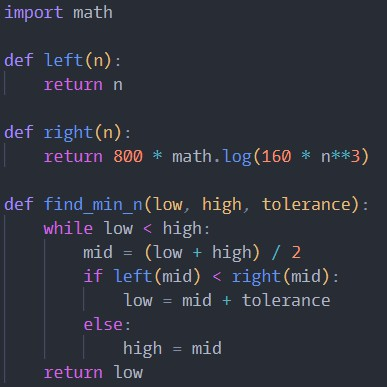
\includegraphics{img/a3_1.jpg}
\end{figure*}
结果为28695.

若$d_{VC}=4, \delta=\epsilon=0.1$

则
\begin{align*}
    n \geq 800 \log(320n^4)
\end{align*}
结果为38393.

若$d_{VC}=5, \delta=\epsilon=0.1$

则
\begin{align*}
    n \geq 800 \log(640n^5)
\end{align*}
结果为48311.

\end{document}
